
%!TEX encoding = UTF-8 Unicode
%!TEX root = ../exercises.tex

\ifPreSolution

\Exercise{\ExeWeekFIVE}\label{exe:W05}

\begin{Goals}
%!TEX encoding = UTF-8 Unicode

%!TEX root = ../compendium2.tex

\item Kunna deklarera klasser med klassparametrar.
\item Kunna skapa objekt med \code{new} och konstruktorargument.
\item Förstå innebörden av referensvariabler och värdet \code{null}.
\item Förstå innebörden av begreppen instans och referenslikhet.
\item Kunna använda nyckelordet \code{private} för att styra synlighet i primärkonstruktor.
\item Förstå i vilka sammanhang man kan ha nytta av en privat konstruktor.
\item Kunna implementera en klass utifrån en specifikation.
\item Förstå skillnaden mellan referenslikhet och strukturlikhet.
\item Känna till hur case-klasser hanterar likhet.
\item Förstå nyttan med att möjliggöra framtida förändring av attributrepresentation.
\item Känna till begreppen getters och setters.
\item Känna till accessregler för kompanjonsobjekt.
\item Känna till skillnaden mellan \code{==} och \code{eq}, samt \code{!=} versus \code{ne}.

\end{Goals}

\begin{Preparations}
\item \StudyTheory{05}
\end{Preparations}

\else


\ExerciseSolution{\ExeWeekFIVE}


\fi


\BasicTasks %%%%%%%%%%%


\WHAT{Para ihop begrepp med beskrivning.}

\QUESTBEGIN

\Task \what

\vspace{1em}\noindent Koppla varje begrepp med den (förenklade) beskrivning som passar bäst:

\begin{ConceptConnections}
  klass & 1 & & A & ett värde som ej refererar till någon instans \\ 
  instans & 2 & & B & nyckelord vid direkt instansiering av klass \\ 
  konstruktor & 3 & & C & ser privata medlemmar i klass med samma namn \\ 
  klassparameter & 4 & & D & binds till argument som ges vid konstruktion \\ 
  referenslikhet & 5 & & E & indirekt åtkomst av attributvärde \\ 
  innehållslikhet & 6 & & F & slipper skriva new; automatisk innehållslikhet \\ 
  case-klass & 7 & & G & instanser anses lika om de har samma tillstånd \\ 
  getter & 8 & & H & indirekt tilldelning av attributvärde \\ 
  setter & 9 & & I & hjälpfunktion för indirekt konstruktonsanrop \\ 
  kompanjonsobjekt & 10 & & J & upplaga av ett objekt med eget tillståndsminne \\ 
  fabriksmetod & 11 & & K & skapar instans, allokerar plats för tillståndsminne \\ 
  \code|null| & 12 & & L & en mall för att skapa flera instanser av samma typ \\ 
  \code|new| & 13 & & M & instanser anses olika även om tillstånden är lika \\ 
\end{ConceptConnections}

\SOLUTION

\TaskSolved \what

\begin{ConceptConnections}
  klass & 1 & ~~\Large$\leadsto$~~ &  I & en mall för att skapa flera instanser av samma typ \\ 
  instans & 2 & ~~\Large$\leadsto$~~ &  F & upplaga av ett objekt med eget tillståndsminne \\ 
  konstruktor & 3 & ~~\Large$\leadsto$~~ &  E & skapar instans, allokerar plats för tillståndsminne \\ 
  klassparameter & 4 & ~~\Large$\leadsto$~~ &  M & binds till argument som ges vid konstruktion \\ 
  referenslikhet & 5 & ~~\Large$\leadsto$~~ &  L & instanser anses olika även om tillstånden är lika \\ 
  innehållslikhet & 6 & ~~\Large$\leadsto$~~ &  J & instanser anses lika om de har samma tillstånd \\ 
  case-klass & 7 & ~~\Large$\leadsto$~~ &  D & slipper skriva new; automatisk innehållslikhet \\ 
  getter & 8 & ~~\Large$\leadsto$~~ &  A & indirekt åtkomst av attributvärde \\ 
  setter & 9 & ~~\Large$\leadsto$~~ &  B & indirekt tilldelning av attributvärde \\ 
  kompanjonsobjekt & 10 & ~~\Large$\leadsto$~~ &  H & ser privata medlemmar i klass med samma namn \\ 
  fabriksmetod & 11 & ~~\Large$\leadsto$~~ &  G & hjälpfunktion för indirekt konstruktonsanrop \\ 
  \code|null| & 12 & ~~\Large$\leadsto$~~ &  K & ett värde som ej refererar till någon instans \\ 
  \code|new| & 13 & ~~\Large$\leadsto$~~ &  C & nyckelord vid direkt instansiering av klass \\ 
\end{ConceptConnections}

\QUESTEND



\WHAT{Klass och instans.}

\QUESTBEGIN

\Task \what~Du har i övning \texttt{\ExeWeekFOUR}~sett hur singelobjekt i en egen namnrymd  kan samla funktioner (metoder) och ha tillstånd (attribut). Men singelobjekt finns bara i en upplaga.
Vill du kunna skapa många objekt av samma typ behöver du en \emph{klass}. En objektupplaga som skapats ur en klass kallas en \emph{instans} av klassen. Varje instans har sitt eget tillstånd.
Deklarera singelobjektet och klassen nedan och klistra in i REPL.

\begin{Code}
object Singelpunkt { var x = 1; var y = 2 }
class  Punkt       { var x = 3; var y = 2 }
\end{Code}

\Subtask  Antag att uttrycken till vänster evalueras uppifrån och ned. Vilket resultat till höger hör ihop med respektive uttryck? Prova i REPL om du är osäker.\footnote{Strängen efter \code{@}-tecknet är en hexadecimal representation av det heltal som tillordnas varje objekt för att systemet ska kunna särskilja olika instanser. \url{https://stackoverflow.com/questions/4712139}}


\begin{ConceptConnections}
  \code|Singelpunkt.x               | & 1 & & A & \code|2| \\ 
  \code|Punkt.x                     | & 2 & & B & \verb|p2: Punkt = Punkt@51ab04bd| \\ 
  \code|val p  = new Singelpunkt    | & 3 & & C & \verb|p1: Punkt = Punkt@27a1a53c| \\ 
  \code|val p1 = new Punkt          | & 4 & & D & \verb|error: not found: type| \\ 
  \code|val p2 = new Punkt          | & 5 & & E & \code|java.lang.NullPointerException| \\ 
  \code|{ p1.x = 1; p2.x }          | & 6 & & F & \code|1| \\ 
  \code|(new Punkt).y               | & 7 & & G & \code|3| \\ 
  \code|{ val p: Punkt = null; p.x }| & 8 & & H & \code|error: not found: value| \\ 
\end{ConceptConnections}

\Subtask Vid tre tillfällen blir det fel. Varför? Är det kompileringsfel eller exekveringsfel?

\SOLUTION

\TaskSolved \what

\SubtaskSolved

\begin{ConceptConnections}
  \code|Singelpunkt.x               | & 1 & ~~\Large$\leadsto$~~ &  E & \code|1| \\ 
  \code|Punkt.x                     | & 2 & ~~\Large$\leadsto$~~ &  A & \code|error: not found: value| \\ 
  \code|val p  = new Singelpunkt    | & 3 & ~~\Large$\leadsto$~~ &  F & \verb|error: not found: type| \\ 
  \code|val p1 = new Punkt          | & 4 & ~~\Large$\leadsto$~~ &  D & \code|p1: Punkt = Punkt@27a1a53c| \\ 
  \code|val p2 = new Punkt          | & 5 & ~~\Large$\leadsto$~~ &  C & \code|p2: Punkt = Punkt@51ab04bd| \\ 
  \code|{ p1.x = 1; p2.x }          | & 6 & ~~\Large$\leadsto$~~ &  G & \code|3| \\ 
  \code|(new Punkt).y               | & 7 & ~~\Large$\leadsto$~~ &  B & \code|2| \\ 
  \code|{ val p: Punkt = null; p.x }| & 8 & ~~\Large$\leadsto$~~ &  H & \code|java.lang.NullPointerException| \\ 
\end{ConceptConnections}

\SubtaskSolved

\noindent\begin{tabular}{l l p{5cm}}

~\\ \emph{fel} & \emph{typ} & \emph{förklaring} \\\hline

\code|value is not a member of object|
& kompileringsfel & det finns ingen instans med namnet \code|Punkt|. \newline \emph{Felmeddelandet syftar på att det i klassens autogenererade konstruktor-ombud saknas en variabel med namnet} \code|x|.\\ % Footnote verkar inte funka, så förklaringen får tyvärr stå i själva tabellen.

\verb|Not found: type|
& kompileringsfel & det finns ingen klass som heter \code|Singelpunkt|\\

\code|NullPointerException|
& körtidsfel & det går inte att referera attribut i en instans som inte finns\\

\end{tabular}

\QUESTEND



\WHAT{Klassparametrar.}

\QUESTBEGIN

\Task \what~Klassen Punkt i föregående uppgift är inte så smidig att använda eftersom man först \emph{efter} instansiering kan ge attributen \code{x} och \code{y} de koordinatvärden man önskar och detta måste ske med explicita tilldelningssatser.

Detta problem kan du lösa med \emph{klassparametrar} som låter dig initialisera attributen med konstruktionsargument och på så sätt ange ett initialtillstånd direkt i samband med instansiering.

Deklarera klassen nedan i REPL.

\begin{Code}
class Point(var x: Int, var y: Int)
\end{Code}


\Subtask  Antag att uttrycken till vänster evalueras uppifrån och ned. Vilket resultat till höger hör ihop med respektive uttryck? Prova i REPL om du är osäker.

\begin{ConceptConnections}
  \code|val p1 = Point(1, 2)        | & 1 & & A & \code|1| \\ 
  \code|val p2 = new Point          | & 2 & & B & \verb|p2: Point = Point@218cf600| \\ 
  \code|val p1 = new Point(1, 2)    | & 3 & & C & \code|error: not found: value| \\ 
  \code|val p2 = new Point(3, 4)    | & 4 & & D & \code|error: too many arguments| \\ 
  \code|p2.x - p1.x                 | & 5 & & E & \code|error: not enough arguments| \\ 
  \code|(new Point(0, 1)).y         | & 6 & & F & \code|2| \\ 
  \code|new Point(0, 1, 2)          | & 7 & & G & \verb|p1: Point = Point@30ef773e| \\ 
\end{ConceptConnections}

\Subtask Vid två tillfällen blir det fel. Varför? Är det kompileringsfel eller exekveringsfel?

\SOLUTION

\TaskSolved \what

\SubtaskSolved

\begin{ConceptConnections}
  \code|val p1 = Point(1, 2)        | & 1 & ~~\Large$\leadsto$~~ &  C & \verb|p1: Point = Point@30ef773e| \\
  \code|val p2 = new Point          | & 2 & ~~\Large$\leadsto$~~ &  B & \verb|missing argument for parameter| \\
  \code|val p2 = new Point(3, 4)    | & 3 & ~~\Large$\leadsto$~~ &  D & \verb|p2: Point = Point@218cf600| \\
  \code|p2.x - p1.x                 | & 4 & ~~\Large$\leadsto$~~ &  F & \code|2| \\
  \code|(new Point(0, 1)).y         | & 5 & ~~\Large$\leadsto$~~ &  A & \code|1| \\
  \code|new Point(0, 1, 2)          | & 6 & ~~\Large$\leadsto$~~ &  E & \verb|too many arguments for constructor|

\end{ConceptConnections}

\SubtaskSolved

\noindent\begin{tabular}{l l p{5cm}}

  ~\\ \emph{fel} & \emph{typ} & \emph{förklaring} \\\hline

  \verb|missing argument for parameter|
  & kompileringsfel  & du måste ge argument vid konstruktion av klassen \code|Point| \\

  \verb|too many arguments for constructor|
  & kompileringsfel & antalet argument stämmer ej överens med antalet klassparametrar\\

\end{tabular}

\QUESTEND



\WHAT{Oföränderlig klass med defaultargument.}

\QUESTBEGIN

\Task \what~Det som gäller för parametrar och argument till funktioner är även tillämpligt på klassparametrar, t.ex. defaultargument och namngivna argument. Man kan \emph{dessutom} framför klassparametrar använda nyckelorden \code{var} och \code{val} och då blir parametern ett synligt attribut. Vill man ha privata attribut kan man ange t.ex. \code{private val} framför klassparameternamnet.
Om inget anges framför en klassparameter är det den allra mest restriktiva synligheten \code{private[this] val} som gäller, vilket innebär att namnet bara syns i den aktuella instansen\footnote{För case-klasser, som vi ska se snart, är det i stället \code{val} medförande synlighet och oföränderlighet som gäller (alltså inte \code{private[this] val}).}.

Deklarera nedan klass i REPL.

\begin{Code}
class Point3D(val x: Int = 0, val y: Int = 0, z: Int = 0)
\end{Code}

\Subtask Antag att uttrycken till vänster evalueras uppifrån och ned. Vilket resultat till höger hör ihop med respektive uttryck? Prova i REPL om du är osäker.

\begin{ConceptConnections}
  \code|val p1 = Point3D()          | & 1 & & A & \code|false| \\ 
  \code|val p2 = Point3D(y = 1)     | & 2 & & B & \code|Reassignment to val| \\ 
  \code|Point3D(z = 2).z            | & 3 & & C & \verb|p1: Point3D = Point3D@2eb37eee| \\ 
  \code|p2.y = 0                    | & 4 & & D & \code|true| \\ 
  \code|p2.y == 0                   | & 5 & & E & \code|value cannot be accessed| \\ 
  \code|p1.x == Point3D().x         | & 6 & & F & \verb|p2: Point3D = Point3D@65a9e8d7| \\ 
\end{ConceptConnections}

\Subtask Vad är problemet med ovan klass om man vill använda den för att representera punkter i 3 dimensioner?

\SOLUTION

\TaskSolved \what~

\SubtaskSolved

\begin{ConceptConnections}
  \code|val p1 = new Point3D        | & 1 & ~~\Large$\leadsto$~~ &  A & \verb|p1: Point3D = Point3D@2eb37eee| \\ 
  \code|val p2 = new Point3D(y = 1) | & 2 & ~~\Large$\leadsto$~~ &  B & \verb|p2: Point3D = Point3D@65a9e8d7| \\ 
  \code|(new Point3D(z = 2)).z      | & 3 & ~~\Large$\leadsto$~~ &  C & \code|error: not found: value| \\ 
  \code|p2.y = 0                    | & 4 & ~~\Large$\leadsto$~~ &  D & \code|error: reassignment to val| \\ 
  \code|p2.y == 0                   | & 5 & ~~\Large$\leadsto$~~ &  F & \code|false| \\ 
  \code|p1.x == (new Point3D).x     | & 6 & ~~\Large$\leadsto$~~ &  E & \code|true| \\ 
\end{ConceptConnections}

\SubtaskSolved Problemet är att så som klassen \code{Point3D} är deklarerad går det inte att avläsa \code{z}-koordinaten efter att en instans konstruerats. Det vore bättre om även \code{z}-attributet är \code{val}.

\QUESTEND



\WHAT{Case-klass, \code{this}, likhet, \code{toString} och kompanjonsobjekt.}

\QUESTBEGIN

\Task \what~\\Klistra in nedan klasser i REPL.

\begin{Code}
case class Pt(x: Int = 0, y: Int = 0):
  def moved(dx: Int = 0, dy: Int = 0): Pt = Pt(x + dx, y + dy)

class MutablePt(private var p: (Int, Int) = (0, 0)):
  def x: Int = p._1
  def y: Int = p._2
  def move(dx: Int = 0, dy: Int = 0) = { p = (x + dx, y + dy); this }
  override def toString = s"MPt($x,$y)"
\end{Code}

\Subtask
Antag att uttrycken till vänster evalueras uppifrån och ned. Vilket REPL-svar till höger hör ihop med respektive uttryck? Prova i REPL om du är osäker.

\begin{ConceptConnections}
  \code|val p1 = Pt(1, 2)             | & 1 & & A & \code|MPt(5,6)| \\ 
  \code|val p2 = Pt(y = 3)            | & 2 & & B & \code|false| \\ 
  \code|val p3 = MutablePt(5, 6)      | & 3 & & C & \code|Pt(0,3)| \\ 
  \code|val p4 = Mutable()            | & 4 & & D & \code|Not found| \\ 
  \code|p2.moved(dx = 1) == Pt(1, 3)  | & 5 & & E & \code|Pt(1,2)| \\ 
  \code|p3.move(dy = 1) == MutablePt(5, 7)| & 6 & & F & \code|true| \\ 
\end{ConceptConnections}

\Subtask Vilken returtyp kommer kompilatorn härleda för funktionen \code{MutablePt.move}?

\Subtask Vad är skillnaden mellan instansiering med universella apply-metoder och instansiering med \code|new|? Finns det något fall där \code|new| måste användas?

\Subtask Vad kallas sådana metoder som \code{ def x } och \code{ def y } ovan?

\SOLUTION

\TaskSolved \what~

\SubtaskSolved

\begin{ConceptConnections}
  \code|val p1 = new Pt(1,2)        | & 1 & ~~\Large$\leadsto$~~ &  G & \code|Pt(1,2)| \\ 
  \code|val p2 = Pt(y=3)            | & 2 & ~~\Large$\leadsto$~~ &  E & \code|Pt(0,3)| \\ 
  \code|val p3 = new MutablePt(5, 6)| & 3 & ~~\Large$\leadsto$~~ &  A & \code|MPt(5,6)| \\ 
  \code|val p4 = Mutable()          | & 4 & ~~\Large$\leadsto$~~ &  F & \code|error: not found: value| \\ 
  \code|p2.moved(dx=1) == Pt(1, 3)  | & 5 & ~~\Large$\leadsto$~~ &  C & \code|true| \\ 
  \code|p3.move(dy=1) == new MutablePt(5,7)| & 6 & ~~\Large$\leadsto$~~ &  B & \code|false| \\ 
  \code|p2 == p3                      | & 7 & ~~\Large$\leadsto$~~ &  D & \verb|warning: always false| \\ 
\end{ConceptConnections}


\SubtaskSolved Kompilatorn härleder \code{MutablePt} eftersom det är typen på självreferensen this.
\begin{REPL}
scala> :type new MutablePt().move()
MutablePt
\end{REPL}

\SubtaskSolved
Instansiering med universella apply-metoder \Eng{universal apply methods} är godis som gör koden enklare att läsa och skriva. Detta är möjligt tack vare att det vid kompilering automatiskt skapas ett konstruktor-ombud \Eng{constructor proxy} som instansierar objektet med nyckelordet \code|new|. Ett konstruktor-ombud är ett kompanjonsobjekt med tillhörande apply-metod.

Ett fall då \code|new| uttryckligen måste användas är vid implementering av egen apply-metod i ett kompanjonsobjekt. Om \code|new| inte används inuti apply-metoden, kommer samma metod att anropas rekursivt istället för att en ny instans skapas. Se följande exempel:

\begin{Code}
class Point3D(val x: Int, val y: Int, val z: Int)

object Point3D:
  var secretNumber = 42
  def apply(x: Int, y: Int, z: Int): Point3D =
    if secretNumber == 42 then
      Point3D(x, y, z) // Koden kommer fastna i en evig loop.

    else new Point3D(x, y, z) // Funkar eftersom 'new' används.
\end{Code}



\SubtaskSolved En metod som avläser (delar av) ett objekts (privata) tillstånd utan att ändra det kallas för en \emph{getter}.

\QUESTEND


\WHAT{Implementera delar av klasserna \code{Pos}, \code{KeyControl}, \code{Mole} och \code{BlockWindow} som behövs under laborationen \hyperref[section:lab:\LabWeekSIX]{\texttt{\LabWeekSIX}}.}

\QUESTBEGIN

\Task\label{exe:classes:labprep}  \what~I nästa laboration ska du bygga vidare på \code{blockmole}-labben och göra ett spel för två spelare där varje spelare styr sin \emph{egen} instans av en \code{blockmole}. Vi måste då göra om \code{Mole} så att den blir en klass i stället för ett singelobjekt. Gör färdigt klasserna nedan och testa noggrant så att de fungerar. 

Alla klasser ska tillhöra \code{package blockbattle} och ligga i varsin egen fil med samma namn som klassen, t.ex. \code{Pos.scala}. 

Tips: Ha ett separat terminalfönster igång och kör Scala CLI med ändringsbevakning enligt nedan kommano. Då kompileras din ändrade kod om automatiskt varje gång du sparar en scala-fil i aktuell katalog.
\begin{REPLnonum}
scala-cli compile . --watch
\end{REPLnonum}
Optionen \code{--watch} kan skrivas kortare med \code{-w} i stället.

\Subtask Under laborationen är det smidigt att kunna representera flyttbara positioner i ett pixelfönster. Implementera case-klassen \code{Pos} i ett nytt terminalfönster enligt nedan så att den fungerar enligt efterföljande REPL-tester.
\scalainputlisting[basicstyle=\ttfamily\fontsize{11}{13}\selectfont]{../workspace/w06_blockbattle/Pos.scala}
Testa så att \code{Pos} fungerar med hjälp av REPL enligt nedan:
\begin{REPL}
> scala-cli repl .
Welcome to Scala 3.3.0 (17.0.6, Java OpenJDK 64-Bit Server VM).
Type in expressions for evaluation. Or try :help.

scala> blockbattle.Pos(1,2)
val res0: blockbattle.Pos = Pos(1,2)

scala> import blockbattle.*

scala> val p = Pos(1,2)
val p: blockbattle.Pos = Pos(1,2)

scala> p.moved(0,1)
val res1: blockbattle.Pos = Pos(1,3)
\end{REPL}
Testa även att anropa \code{moved} på klassnamnet, t.ex. \code{Pos.moved(0,1)}. Fungerar detta? Varför/varför inte? Hur skiljer sig anrop till metoder i singelobjekt respektive klassinstanser?

\Subtask Under laborationen är det smidigt att kunna representera vilka tangenter som motsvarar de olika riktningar som en användare kan styra sin mullvad i. Gör klart case-klassen \code{KeyControl} enligt nedan så att den fungerar enligt efterföljande REPL-tester. Metoden \code{direction} ska ge ett delta-steg i rätt \code{(x, y)}-riktning för ett givet tangentnamn. Metoden \code{has} ska ge \code{true} om tangentnamnet finns i någon av de fyra riktningstangenterna i denna denna \code{KeyControl}-instans, annars \code{false}.
\scalainputlisting[basicstyle=\ttfamily\fontsize{10}{12}\selectfont]{../workspace/w06_blockbattle/KeyControl.scala}
% \begin{CodeSmall}
% case class KeyControl(left: String, right: String, up: String, down: String){
%   def direction(key: String): (Int, Int) = ???
%
%   def has(key: String): Boolean = ???
% }
% \end{CodeSmall}
\begin{REPL}
scala> import blockbattle.*

scala> val kc1 = KeyControl(right="d",left="a",up="w",down="s")
val kc1: blockbattle.KeyControl = KeyControl(a,d,w,s)

scala> val kc2 = KeyControl("Left","Right","Up","Down")
val kc2: blockbattle.KeyControl = KeyControl(Left,Right,Up,Down)

scala> kc2.left
val res0: String = Left

scala> kc2.has("a")
val res1: Boolean = false

scala> kc2.has("Up")
val res2: Boolean = true

scala> kc1.direction("a")
val res3: (Int, Int) = (-1,0)

scala> kc1.direction("s")
val res4: (Int, Int) = (0,1)

scala> kc1.direction("d")
val res5: (Int, Int) = (1,0)

scala> kc1.direction("w")
val res6: (Int, Int) = (0,-1)

scala> Pos(1,2).moved(kc1.direction("a"))
val res7: blockbattle.Pos = Pos(0,2)
\end{REPL}


\Subtask Gör klart klassen \code{Mole} enligt nedan. Mole är en klass som representerar en blockmullvad med föränderliga attribut för position, riktning och poäng. Varje instans har även oföränderliga attribut som håller reda på dess namn, dess färg och vilka tangenter som kan användas för att styra mullvaden. Implementera klassens medlemmar en i taget och testa noga med lämpliga testfall efter varje tillägg/buggfix. Skapa ett huvudprogram t.ex. i filen \code{Main.scala} med dina tester som skapar instanser och skriver ut attribut etc. 
\scalainputlisting[basicstyle=\ttfamily\fontsize{10}{12}\selectfont]{../workspace/w06_blockbattle/Mole.scala}
% \begin{CodeSmall}
% class Mole(
%   val name: String,
%   var pos: Pos,
%   var dir: (Int, Int),
%   val color: java.awt.Color,
%   val keyControl: KeyControl
% ){
%   var points = 0
%
%   override def toString =
%     s"Mole[name=$name, pos=$pos, dir=$dir, points=$points]"
%
%   /** Om keyControl.has(key) så uppdateras riktningen dir enligt keyControl */
%   def setDir(key: String): Unit = ???
%
%   /** Uppdaterar dir till motsatta riktningen */
%   def reverseDir(): Unit = ???
%
%   /** Uppdaterar pos så att den blir nextPos */
%   def move(): Unit = ???
%
%   /** Ger nästa position enligt riktningen dir utan att uppdatera pos */
%   def nextPos: Pos = ???
% }
% \end{CodeSmall}



\Subtask Under laborationen behöver du en klass \code{blockbattle.BlockWindow} som med hjälp av \code{introprog.PixelWindow} erbjuder blockgrafik. Varje instans av \code{BlockWindow} ska ha ett attribut som refererar till en \code{PixelWindow}-instans. Detta kallas \textbf{aggregering} \Eng{aggregation}.\footnote{\url{https://en.wikipedia.org/wiki/Object\_composition\#Aggregation}}

För att det ska gå att kompilera och testa din \code{BlockWindow}-klass behöver du ha \code{introprog}-paketet på classpath. Ladda ner filen \url{https://fileadmin.cs.lth.se/introprog.jar} via din webbläsare eller med kommandot \code{curl} nedan (notera att det är stora bokstaven \code{O} och inte en nolla i optionen \code{-sLO}):

\begin{REPLnonum}
curl -o introprog.jar -sLO  https://fileadmin.cs.lth.se/introprog.jar
scala-cli run . --jar introprog.jar
\end{REPLnonum}
Då hamnar \code{introprog.jar} automatiskt på classpath. 
% Du kan också köra igång ditt program ''manuellt'' med detta kommando (semikolon i Windows):
% \begin{REPLnonum}
% > scala -cp "lib/introprog.jar:target/scala-3.0.1/classes" blockbattle.Main
% \end{REPLnonum}

Gör klart klassen \code{BlockWindow} enligt nedan. Metoden \code{setBlock} ska med hjälp av metoden \code{pixelWindow.fill} fylla ett kvadratiskt område med sidan \code{blockSize} pixlar på en viss position \code{pos} i block-koordinater och med en viss färg \code{color}. Metoden \code{getBlock} ska med hjälp av metoden \code{pixelWindow.getPixel} ge färgen för övre vänstra hörnet i blocket på position \code{pos} i block-koordinater.
\scalainputlisting[basicstyle=\ttfamily\fontsize{10}{12}\selectfont]{../workspace/w06_blockbattle/BlockWindow.scala}
% \begin{CodeSmall}
% class BlockWindow(
%   val nbrOfBlocks: (Int, Int),
%   val title: String = "BLOCK WINDOW",
%   val blockSize: Int = 14
% ) {
%   import introprog.PixelWindow
%
%   val pixelWindow = new PixelWindow(
%     nbrOfBlocks._1 * blockSize, nbrOfBlocks._2 * blockSize, title)
%
%   def setBlock(pos: Pos, color: java.awt.Color): Unit = ???
%
%   def getBlock(pos: Pos): java.awt.Color = ???
%
%   def write(
%     text: String,
%     pos: Pos,
%     color: java.awt.Color,
%     textSize: Int = blockSize
%   ): Unit = pixelWindow.drawText(
%       text, pos.x * blockSize, pos.y * blockSize, color, textSize)
%
%   def nextEvent(maxWaitMillis: Int = 10): BlockWindow.Event.EventType  = {
%     import BlockWindow.Event._
%     pixelWindow.awaitEvent(maxWaitMillis)
%     pixelWindow.lastEventType match {
%       case PixelWindow.Event.KeyPressed   => KeyPressed(pixelWindow.lastKey)
%       case PixelWindow.Event.WindowClosed => WindowClosed
%       case _                              => Undefined
%     }
%   }
% }
%
% object BlockWindow {
%   def delay(millis: Int): Unit = Thread.sleep(millis)
%
%   object Event {
%     trait EventType
%     case class  KeyPressed(key: String) extends EventType
%     case object WindowClosed            extends EventType
%     case object Undefined               extends EventType
%   }
% }
% \end{CodeSmall}
I instruktionerna till laborationen \texttt{\LabWeekSIX} finns tips om hur du kan hantera händelser i ett \code{BlockWindow} med hjälp av metoden \code{nextEvent} ovan.

\Subtask Gör så att huvudprogrammet i \code{Main.scala} ritar några valfria block i en instans av klassen \code{BlockWindow}. Skapa även en \code{while (!quit)}-loop som med hjälp av \code{nextEvent()} skriver ut händelser i terminalen som inte är av typen \code{Undefined}. 

Metoden \code{nextEvent()} ligger i klassen \code{BlockWindow}. Varje looprunda ska även innehålla en \code{200} millisekunders fördröjning genom anrop av \code{delay}-metoden som definierats i kompanjonsobjektet \code{BlockWindow} ovan. Om händelsen \code{WindowClosed} inträffar ska loopen avslutas. Kör huvudprogrammet och kontrollera så att resultatet blir som förväntat.

\SOLUTION


\TaskSolved \what Denna uppgift är laborationsförberedelse. Utvärdera dina lösningar genom egna tester i REPL.

\SubtaskSolved Det går inte att anropa \code{Pos.moved(0,1)}. Anledningen till detta är att \code{moved} inte existerar i kompanjonsobjektet \code{Pos}, därav felmeddelandet ''value \code{moved} is not a member of object \code{Pos}''. För att anropa en metod definierad inuti en klass måste man göra anropet via en (referens till en) instans av klassen.

\QUESTEND





%\clearpage

\ExtraTasks %%%%%%%%%%%%%%%%%%%%%%%%%%%%%%%%%%%%%%%%%%%%%%%%%%%%%%%%%%%%%%%%%%%%


\WHAT{Instansiering med \code{new} och värdet \code{null}.}

\QUESTBEGIN

\Task  \what~  Man skapar instanser av klasser med \code{new}. Då anropas konstruktorn och plats reserveras i datorns minne för objektet. Variabler av referenstyp som inte refererar till något objekt har värdet \code{null}.

\Subtask Vad händer nedan? Vilka rader ger felmeddelande och i så fall hur lyder felmeddelandet?

\begin{REPL}
scala> class Gurka(val vikt: Int)
scala> var g: Gurka = null
scala> g.vikt
scala> g = new Gurka(42)
scala> g.vikt
scala> g = null
scala> g.vikt
\end{REPL}

\Subtask Rita minnessituationen efter raderna 2, 4, 6.

\SOLUTION


\TaskSolved \what


\SubtaskSolved  Rad 3 och 7 ger båda felmeddelandet \code{java.lang.NullPointerException},  på grund av försök att referera medlemmar med hjälp av en \code{null}-referens, som alltså inte pekar på något objekt.

\SubtaskSolved  \includegraphics[scale=0.6]{../img/w06-solutions/1b}


\QUESTEND



\WHAT{Skapa en punktklass som kan hantera polära koordinater.}

\QUESTBEGIN

\Task \what~
Du ska skapa en oföränderlig case-klass \code{Point} som kan representera en koordinat både med ''vanliga'' kartesiska koordinater\footnote{\url{https://sv.wikipedia.org/wiki/Kartesiskt_koordinatsystem}} och med polära koordinater%
\footnote{\url{https://sv.wikipedia.org/wiki/Pol\%C3\%A4ra\_koordinater}}.

\Subtask Skapa kod med hjälp av en editor, t.ex. VS \code{code}, i filen  \code{Point.scala} enligt följande riktlinjer:
\begin{enumerate}[noitemsep]
\item \code{Point} ska ligga i paketet \code{graphics}.

\item \code{Point} ska ha följande två publika, oföränderliga klassparametrar:
\begin{itemize}[nolistsep, noitemsep]
\item \code{x: Double} för x-koordinaten.
\item \code{y: Double} för y-koordinaten.
\end{itemize}

\item \code{Point} ska ha följande publika medlemmar (två oföränderliga attribut och en metod):
\begin{itemize}[nolistsep, noitemsep]
\item \code{lazy val r: Double} ska ge motsvarande polära koordinatens
 avstånd till origo.
\item \code{lazy val theta: Double} ska ge polära koordinatens vinkel i radianer.
\item \code{def +(p: Point): Point} ska ge en ny punkt vars koordinat är summan av x- respektive y-koordinaterna för denna instans och punkten \code{p}.
\end{itemize}

\item \code{Point} ska ha ett kompanjonsobjekt med en metod som konstruerar en punkt från polära koortdinater. Metoden ska ha detta huvud: \\\code{def polar(r: Double, theta: Double): Point}

\end{enumerate}

\noindent Tips:
\begin{itemize}
\item Du har nytta av metoderna $r = $ \code{math.hypot(x, y)} och $\theta = $ \code{math.atan2(y, x)} vid omvandling till polära koordinater:

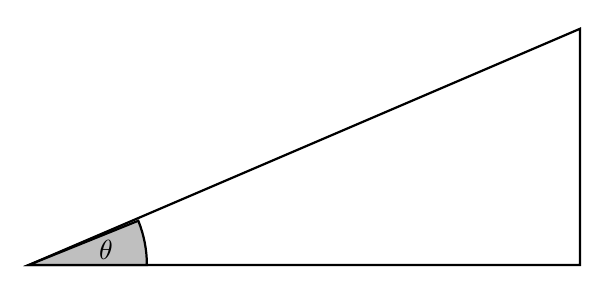
\begin{tikzpicture}[thick]
\coordinate (O) at (0,0);
\coordinate (A) at (7,0);
\coordinate (B) at (7,3);
\draw (O)--(A)--(B)--cycle;

%\tkzLabelSegment[below=2pt](O,A){\textit{adjacent leg}}
%\tkzLabelSegment[left=2pt](O,B){\textit{hypotenuse}}
%\tkzLabelSegment[above right=2pt](A,B){\textit{opposite leg}}

\tkzLabelSegment[below=5pt](O,A){\textit{x}}
\tkzLabelSegment[above left=5pt](O,B){\textit{r}}
\tkzLabelSegment[right=5pt](A,B){\textit{y}}

%\tkzMarkAngle[fill= orange,size=1.5cm, opacity=.4](A,O,B)
%\tkzLabelAngle[pos = 2](A,O,B){\texttt{$\theta$}}
 %%% AAAARGH ovan slutade funka så gjorde nedan HACK i stället
 \draw[fill=lightgray, thick] (0,0) -- (0:1.5cm) arc (0:22:1.5cm) node at (11:1.0cm) {$\theta$} -- cycle;

% \tkzMarkAngle[fill= orange,size=0.65cm, opacity=.4](A,O,B)
% \tkzLabelAngle[pos = 0.35](A,O,B){$\gamma$}
%
% \tkzMarkAngle[fill= orange,size=0.8cm, opacity=.4](B,A,O)
% \tkzLabelAngle[pos = 0.6](B,A,O){$\alpha$}
%
% \tkzMarkAngle[fill= orange,size=0.7cm, opacity=.4](O,B,A)
% \tkzLabelAngle[pos = 0.5](O,B,A){$\beta$}

\end{tikzpicture}

\item Du har nytta av metoderna \code{math.cos(theta)} och \code{math.sin(theta)} vid omvandling från polära koordinater.

\item Notera att klassens attribut är av typen \code{Double} och inte \code{Int}, trots att vi senare ska använda punkten för att beskriva en diskret pixelposition i ett \code{PixelWindow}. Anledningen till detta är att det kan uppstå avrundningsfel vid numeriska beräkningar. Detta blir särskilt märkbart vid upprepad räkning med små värden, t.ex. när man ritar en approximerad cirkel med många linjesegment.
\end{itemize}

\Subtask Studera nu följande singelobjekt \code{PolygonWindow} som med hjälp av ett \code{PixelWindow} ger möjlighet att rita ut polygoner:
\begin{Code}
object PolygonWindow:
  import introprog.PixelWindow
  import java.awt.Color

  val black = Color(0,0,0)
  val coolGreen = Color(0,255,100)
  val width = 500
  val height = 500
  val window = PixelWindow(width, height, title = "Polygons", background = black, foreground = coolGreen)

  private def convertPoint(point: Point): Vector[Int] = 
    Vector(point.x.toInt, point.y.toInt)

  def draw(polygon: Polygon): Unit =
    for i <- 0 until polygon.nbrOfCorners do
      val from = convertPoint(polygon.pointsForDrawing(i)).map(_ + width/2)
      val to = convertPoint(polygon.pointsForDrawing((i+1) % polygon.nbrOfCorners)).map(_ + width/2)
      window.line(from(0), from(1), to(0), to(1), lineWidth = 2)
\end{Code}
Skapa case-klassen \code{Polygon(points: Vector[Point], midPoint: Point)} med attributen \code{lazy val nbrOfCorners: Int} och \code{lazy val pointsForDrawing: Vector[Point]} så att ovanstående kod går att köra.
\code{Polygon} ska ha ett kompanjonsobjekt med en metod \code{makePolygon(nbrOfCorners: Int, radius: Double, midPoint: Point): Polygon} för att skapa polygoner.

\SOLUTION

\TaskSolved \what~

\Subtask \begin{Code}
package graphics

case class Point(x: Double, y: Double):
  lazy val r: Double          = math.hypot(x, y)
  lazy val theta: Double      = math.atan2(y, x)
  def +(p: Point): Point = Point(x + p.x, y + p.y)

object Point:
  def polar(r: Double, theta: Double): Point =
    Point(r * math.cos(theta), r * math.sin(theta))
\end{Code}

\Subtask \begin{Code}
case class Polygon(points: Vector[Point], midPoint: Point):
  lazy val nbrOfCorners: Int = points.length
  lazy val pointsForDrawing: Vector[Point] = points.map(_ + midPoint)
  
object Polygon:
  def makePolygon(nbrOfCorners: Int, radius: Double, midPoint: Point): Polygon =
    val points = new Array[Point](nbrOfCorners)
    for i <- 0 until nbrOfCorners do
      val theta = i * (2 * math.Pi) / nbrOfCorners
      points(i) = Point.polar(radius, theta)
    end for
    Polygon(points.toVector, midPoint)
\end{Code}


\QUESTEND




\WHAT{Klasser, instanser och skräp.}

\QUESTBEGIN

\Task  \what~För länge sedan i en galax långt långt borta...

\begin{Code}
case class Arm(ärTillVänster: Boolean)

case class Ben(ärTillVänster: Boolean)

case class Huvud(harHår: Boolean = true)

case class Rymdvarelse(
      arm1:   Arm   = Arm(true),
      arm2:   Arm   = Arm(false),
      ben1:   Ben   = Ben(true),
      ben2:   Ben   = Ben(false),
      huvud1: Huvud = Huvud(harHår = false),
  var huvud2: Huvud = Huvud()
):
  def ärSkallig = !huvud1.harHår && !huvud2.harHår
\end{Code}

\Subtask Klistra in ovan rymdkod i REPL och evaluera nedan rader. Rita minnessituationen efter rad 5 och beskriv vad som händer.
\begin{REPL}
scala> val alien = Rymdvarelse()
scala> alien.ärSkallig
scala> val predator = Rymdvarelse()
scala> predator.ärSkallig
scala> predator.huvud2 = alien.huvud1
scala> predator.huvud2 eq alien.huvud1  // test av referenslikhet
scala> println(predator)
scala> predator.ärSkallig
\end{REPL}

\Subtask Vad händer så småningom med det ursprungliga \code{huvud2}-objektet i predator efter tilldelningen på rad 5? Går det att referera till detta objekt på något sätt?

\SOLUTION

\TaskSolved \what

\SubtaskSolved  Vi skapar två rymdvarelser, \code{alien} och \code{predator}, med vardera två ben och två armar, samt vardera två huvuden (där det ena är skalligt och det andra har hår). Efter det är varken \code{alien} eller \code{predator} skallig eftersom båda har ett huvud med hår. Sen låter man referensen till \code{predator}s huvud med hår referera till aliens huvud utan hår. Nu är predator helt skallig och delar huvud med alien.

\includegraphics[scale=0.65]{../img/w06-solutions/2b}

\SubtaskSolved  Eftersom det inte längre finns någon referens som pekar på det objektet kommer skräpsamlaren att ta hand om det och det kommer förr eller senare skrivas över av något annat när platsen i minnet behövs. Objekt som inte har någon referens till sig går inte att komma åt.

\QUESTEND




\WHAT{Case-klass. Oföränderlig kvadrat.}

\QUESTBEGIN

\Task \label{task:Square} \what~

\Subtask Implementera nedan kvadrat med en editor och klistra in den i REPL.

\begin{Code}
case class Square(val x: Int = 0, val y: Int = 0, val side: Int = 1):
  val area: Int = ???

  /** Creates a new Square moved to position (x + dx, y + dy) */
  def moved(dx: Int, dy: Int): Square = ???

  def isEqualSizeAs(that: Square): Boolean = ???

  /** Multiplies the side with factor and rounded to nearest integer */
  def scale(factor: Double): Square = ???

object Square:
  /** A Square at (0, 0) with side 1 */
  val unit: Square = ???
\end{Code}

\Subtask Testa din kvadrat enligt nedan. Förklara vad som händer.

\begin{REPL}
scala> val (s1, s2) = (Square(), Square(1, 10, 1))
scala> val s3 = s1 moved (1,-5)
scala> s1 isEqualSizeAs s3
scala> s2 isEqualSizeAs s1
scala> s1 isEqualSizeAs Square.unit
scala> s2.scale(math.Pi) isEqualSizeAs s2
scala> s2.scale(math.Pi) isEqualSizeAs s2.scale(math.Pi)
scala> s2.scale(math.Pi) eq s2.scale(math.Pi)
scala> Square.unit eq Square.unit
\end{REPL}

\SOLUTION

\TaskSolved \what

\SubtaskSolved

\begin{Code}
case class Square(val x: Int = 0, val y: Int = 0, val side: Int = 1):
  val area: Int = side * side

  def moved(dx: Int, dy: Int): Square = Square(x + dx, y + dy, side)

  def isEqualSizeAs(that: Square): Boolean = this.side == that.side

  def scale(factor: Double): Square =
    Square(x, y, (side * factor).round.toInt)

object Square:
  val unit: Square = Square()
\end{Code}

\SubtaskSolved
\begin{REPL}
scala> val (s1, s2) = (Square(), Square(1, 10, 1))
val s1: Square = Square(0,0,1)
val s2: Square = Square(1,10,1)

scala> val s3 = s1 moved (1,-5)
val s3: Square = Square(1,-5,1)

scala> s1 isEqualSizeAs s3       // lika storlek
val res0: Boolean = true

scala> s2 isEqualSizeAs s1       // lika storlek
val res1: Boolean = true

scala> s1 isEqualSizeAs Square.unit   // s1 har sidan 1
val res2: Boolean = true

scala> s2.scale(math.Pi) isEqualSizeAs s2  // olika storlek
val res3: Boolean = false

scala> s2.scale(math.Pi) == s2.scale(math.Pi) // lika innehåll
val res4: Boolean = true

scala> s2.scale(math.Pi) eq s2.scale(math.Pi)  // olika objekt
val res5: Boolean = false

scala> Square.unit eq Square.unit   // samma objekt
val res6: Boolean = true
\end{REPL}

\QUESTEND




\clearpage

\AdvancedTasks %%%%%%%%%%%%%%%%%%%%%%%%%%%%%%%%%%%%%%%%%%%%%%%%%%%%%%%%%%%%%%%%%

\WHAT{Innehållslikhet mellan olika typer.}

\QUESTBEGIN

\Task \what~Klistra in nedan klasser i REPL och undersök vad som händer.

\begin{Code}
class Gurka(val vikt: Int)

class Bil(val typ: String)
\end{Code}

\begin{REPL}
scala> class Gurka(val vikt: Int)
     |
     | class Bil(val typ: String)
// defined class Gurka
// defined class Bil

scala> 42 == "Fyrtiotvå"

scala> Gurka(50) == Bil("Sedan")

\end{REPL}

Finns det något resultat som är problematiskt, och i så fall, varför?


\SOLUTION

\TaskSolved \what~
\begin{REPL}
scala> 42 == "Fyrtiotvå"
1 |42 == "Fyrtiotvå"
  |^^^^^^^^^^^^^^^^^
  |Values of types Int and String cannot be compared with == or !=

scala> Gurka(50) == Bil("Sedan")
val res0: Boolean = false
\end{REPL}

Det andra uttrycket är problematiskt eftersom det alltid kommer resultera i \code|false|, då klasserna \code|Gurka| och \code|Bil| är två ojämförbara typer som inte bör jämföras med avseende på innehållslikhet. Detta försämrar typsäkerheten vilket ökar risken för svårupptäckta buggar där fel typer jämförs.

Likhetsjämförelser som sker mellan primitiva typer typkollas av kompilatorn och kan därför ge kompileringsfel om två olika typer, såsom \code|Int| och \code|String|, jämförs med varandra. Detta gäller dock i regel inte egendefinierade typer, vilket alltså innebär att en likhetsjämförelse mellan olika egendefinierade typer alltid resulterar i \code|false|.

Det är emellertid möjligt att få samma typkoll för egendefinierade typer som för primitiva typer genom att importera \code|scala.language.strictEquality|.

\begin{Code}
import scala.language.strictEquality
class Gurka(val vikt: Int)

class Bil(val typ: String)
\end{Code}

\begin{REPL}
scala> Gurka(50) == Bil("Sedan")
1 |Gurka(50) == Bil("Sedan")
  |^^^^^^^^^^^^^^^^^^^^^^^^^
  |Values of types Gurka and Bil cannot be compared with == or !=
\end{REPL}

\QUESTEND


\WHAT{Attributrepresentation. Privat konstruktor. Fabriksmetod.}

\QUESTBEGIN

\Task \what~Kim Kodkunnig skapade för länge sedan denna klass som används på många ställen i befintlig kod:

\begin{Code}
class Point private (val x: Int, val y: Int)
object Point:
  def apply(x: Int = 0, y: Int = 0): Point = new Point(x, y)
  val origo = apply()
\end{Code}

\Subtask Vad händer om du försöker instansiera Kim Kodkunnigs klass direkt med nyckelordet \code{new}?

\Subtask Varför använder Kim Kodkunnig ett kompanjonsobjekt med en fabriksmetod? Vilka accessregler gäller mellan ett kompanjonsobjekt och klassen med samma namn?

\Subtask Hjälp Kim Kodkunnig att ändra attributrepresentationen så att det oföränderliga tillståndet utgörs av en 2-tupel \code{val p: (Int, Int)} i stället. Befintlig kod ska inte behöva ändras och klassen \code{Point} ska bete sig från ''utsidan'' precis som innan.

\SOLUTION

\TaskSolved \what~

\SubtaskSolved Det blir kompileringsfel eftersom konstruktorn är privat.
\begin{REPL}
scala> class Point private (val x: Int, val y: Int)
     | object Point:
     |   def apply(x: Int = 0, y: Int = 0): Point = new Point(x, y)
     |   val origo = apply()
     |
// defined class Point
// defined object Point

scala> new Point(0, 0)
1 |new Point(0, 0)
  |    ^^^^^
  |constructor Point cannot be accessed as a member of Point from module class
\end{REPL}

\SubtaskSolved
\begin{itemize}
  \item Genom att ha en privat konstruktor och bara göra indirekt instansiering via fabriksmetod är lätt ändra attributrepresentation i framtiden utan att befintlig kod behöver ändras.

  \item Accessreglerna för kompanjonsobjekt är sådana att kompanjoner ser varandras privata delar.
\end{itemize}

\SubtaskSolved

\begin{Code}
class Point private (private val p: (Int, Int)):
  def x: Int = p._1
  def y: Int = p._2

object Point:
  def apply(x: Int = 0, y: Int = 0): Point = new Point(x, y)
  val origo = apply()
\end{Code}

\QUESTEND



\WHAT{Synlighet av klassparametrar och konstruktor, \code{private[this]}.}

\QUESTBEGIN

\Task  \what~

\Subtask En av gurk-klasserna nedan är trasig. Varför och vad blir det för fel?

\begin{Code}
class Gurka1(vikt: Int)

class Gurka2(val vikt: Int)

class Gurka3(private val vikt: Int)

class Gurka4(private val vikt: Int, kompis: Gurka4):
  def kompisVikt = kompis.vikt

class Gurka5(private[this] val vikt: Int, kompis: Gurka5):
  def kompisVikt = kompis.vikt

class Gurka6 private (vikt: Int)

class Gurka7 private (var vikt: Int)
object Gurka7:
  def apply(vikt: Int) =
    require(vikt >= 0, "negativ vikt: " + vikt)
    new Gurka7(vikt)
\end{Code}

\Subtask Undersök nedan vad nyckelorden \code{val} och \code{private} får för konsekvenser. Förklara vad som händer. Vilka rader ger vilka felmeddelanden?

\begin{REPL}
scala> new Gurka1(42).vikt
scala> new Gurka2(42).vikt
scala> new Gurka3(42).vikt
scala> val ingenGurka: Gurka4 = null
scala> new Gurka4(42, ingenGurka).kompisVikt
scala> new Gurka4(42, new Gurka4(84, null)).kompisVikt
scala> new Gurka6(42)
scala> new Gurka7(-42)
scala> Gurka7(-42)
scala> val g = Gurka7(42)
scala> g.vikt
scala> g.vikt = -1
scala> g.vikt
\end{REPL}


\SOLUTION


\TaskSolved \what

\SubtaskSolved \code{Gurka5} är trasig. Eftersom vikten i \code{Gurka5} är privat för instansen och inte klassen, kan en instans inte accessa en annan instans vikt.
\begin{REPL}
11 |  def kompisVikt = kompis.vikt
   |                   ^^^^^^^^^^^
   |value vikt cannot be accessed as a member of (Gurka5.this.kompis : Gurka5) from class Gurka5.
\end{REPL}


\SubtaskSolved
\begin{REPL}
scala> new Gurka1(42).vikt
1 |new Gurka1(42).vikt
  |^^^^^^^^^^^^^^^^^^^
  |value vikt cannot be accessed as a member of Gurka1 from module class

scala> new Gurka2(42).vikt
val res0: Int = 42

scala> new Gurka3(42).vikt
1 |new Gurka3(42).vikt
  |^^^^^^^^^^^^^^^^^^^
  |value vikt cannot be accessed as a member of Gurka3 from module class

scala> val ingenGurka: Gurka4 = null
val ingenGurka: Gurka4 = null

scala> new Gurka4(42, ingenGurka).kompisVikt
java.lang.NullPointerException: Cannot invoke "rs$line$1$Gurka4.vikt()" bec...
  at rs$line$1$Gurka4.kompisVikt(rs$line$1:8)
  ... 38 elided

scala> new Gurka4(42, new Gurka4(84, null)).kompisVikt
val res2: Int = 84

scala> new Gurka6(42)
1 |new Gurka6(42)
  |    ^^^^^^
  |constructor Gurka6 cannot be accessed as a member of Gurka6 from module...

scala> new Gurka7(-42)
1 |new Gurka7(-42)
  |    ^^^^^^
  |constructor Gurka7 cannot be accessed as a member of Gurka7 from module...

scala> Gurka7(-42)
java.lang.IllegalArgumentException: requirement failed: negativ vikt: -42

scala> val g = Gurka7(42)
val g: Gurka7 = Gurka7@51fd1c7c

scala> g.vikt
val res4: Int = 42

scala> g.vikt = -1

scala> g.vikt
val res5: Int = -1
\end{REPL}

\QUESTEND





\WHAT{Egendefinierad setter kombinerat med privat konstruktor.}

\QUESTBEGIN

\Task  \what~Klistra in denna kod i REPL:

\begin{Code}
class Gurka8 private (private var _vikt: Int):
  def vikt = _vikt
  def vikt_=(v: Int): Unit =
    require(v >= 0, "negativ vikt: " +v)
    _vikt = v

object Gurka8:
  def apply(vikt: Int) =
    require(vikt >= 0, "negativ vikt: " + vikt)
    new Gurka8(vikt)
\end{Code}


\Subtask Förklara vad som händer nedan. Vilka rader ger vilka felmeddelanden?
\begin{REPL}
scala> val g = Gurka8(-42)
scala> val g = Gurka8(42)
scala> g.vikt
scala> g.vikt = 0
scala> g.vikt = -1
scala> g.vikt += 42
scala> g.vikt -= 1000
\end{REPL}

\Subtask Vad är fördelen med möjligheten att skapa egendefinierade setters?

\SOLUTION


\TaskSolved \what


\SubtaskSolved

Rad 1:
\begin{REPL}
	java.lang.IllegalArgumentException: requirement failed: negativ vikt: -42
\end{REPL}
\code{Gurka8.apply} kräver att \code{vikt >= 0} annars kastar \code{require} ett undantag.

Rad 5:
\begin{REPL}
	java.lang.IllegalArgumentException: requirement failed: negativ vikt: -1
\end{REPL}
Settern \code{vikt_=} kräver att \code{vikt >= 0} annars kastar \code{require} ett undantag.

Rad 7:
\begin{REPL}
	java.lang.IllegalArgumentException: requirement failed: negativ vikt: -958
\end{REPL}
Eftersom \code{42 - 1000} är mindre än noll kastar \code{require} ett undantag.

\SubtaskSolved  Man kan sätta egna mer specifika krav på vad som får göras med värdena så man har större koll på att inget oväntat händer.

\QUESTEND




\WHAT{Objekt med föränderligt tillstånd \Eng{mutable state}.}

\QUESTBEGIN

\Task  \what~  Du ska implementera en modell av en hoppande groda som uppfyller följande krav:
\begin{enumerate}%[nolistsep, noitemsep]
\item Varje grodobjekt ska hålla reda på var den är.
\item Varje grodobjekt ska hålla reda på hur långt grodan hoppat totalt.
\item Varje grodobjekt ska kunna beräkna hur långt det är mellan grodans nuvarande position och utgångsläget.
\item Alla grodor börjar sitt hoppande i origo.
\item En groda kan hoppa enligt två metoder:
  \begin{itemize} [nolistsep, noitemsep]
  \item relativ förflyttning enligt parametrarna \code{dx} och \code{dy},
  \item slumpmässig relativ förflyttning $[1, 10]$ i x-ledsförändring och $[1, 10]$ i y-ledsförändring.
  \end{itemize}
\end{enumerate}

\Subtask Implementera klassen \code{Frog} enligt nedan kodskelett och ovan krav.

\begin{Code}
class Frog private (initX: Int = 0, initY: Int = 0):
  def x: Int = ???
  def y: Int = ???

  def jump(dx: Int, dy: Int): Unit = ???
  def randomJump: Unit = ???

  def distanceToStart: Double = ???
  def distanceJumped: Double = ???
  def distanceTo(that: Frog): Double = ???

object Frog:
  def spawn(): Frog = ???
\end{Code}
\emph{Tips:}
\begin{itemize} [nolistsep, noitemsep]
\item Om namnet man vill ge ett privat föränderligt attribut ''krockar'' med ett metodnamn, är det vanligt att man börjar attributets namn med understreck, t.ex. \code{private var _x } för att på så sätt undkomma namnkonflikten.
\item Inför en metod i taget och klistra in den nya grodan i REPL efter varje utvidgning och testa.
\end{itemize}



\Subtask Skapa en metod \code{def test(): Unit} i ett singelobjekt \code{FrogTest} som innehåller kod som gör minst en kontroll av varje krav. Om ingen kontroll går fel ska \code{"Test Ok!"} skrivas ut, annars ska exekveringen avbrytas. \emph{Tips:} Använd \code{assert(b, msg)} som avbryter exekveringen och skriver ut \code{msg} om \code{b} är falsk.

\Subtask Vad kallas en metod som enbart returnerar värdet av ett privat attribut?

\Subtask Inför setters för attributen som håller reda på x- och y-postitionen. Förändringar av positionen i x- eller y-led ska räknas som ett hopp och alltså registreras i det attribut som håller reda på det ackumulerade hoppavståndet.

\Subtask Simulera ett massivt grodhoppande med krockdetektering genom att skapa 100 grodor som till att börja med är placerade på x-axeln med avståndet $8$ längdenheter mellan sig. För varje runda i en \code{while}-sats, låt en slumpässigt vald groda göra ett \code{randomJump} tills någon groda befinner sig närmare än $0.5$ längdenheter, vilket är definitionen på att de har krockat. Räkna hur många looprundor som behövs innan något grodpar krockar och skriv ut antalet. Skriv även ut det totala antalet \\ \emph{Tips:} Börja med pseudokod på papper. Använd en grodvektor.


\SOLUTION


\TaskSolved \what


\SubtaskSolved
\begin{Code}
class Frog private (initX: Int = 0, initY: Int = 0):
  private var _x: Int = initX
  private var _y: Int = initY
  private var _distanceJumped: Double = 0

  def x: Int = _x
  def y: Int = _y

  def jump(dx: Int, dy: Int): Unit =
    _x += dx
    _y += dy
    _distanceJumped += math.hypot(dx, dy)


  def randomJump: Unit =
    def rnd = util.Random.nextInt(10) + 1
    jump(rnd, rnd)

  def distanceToStart: Double = math.hypot(x,y)
  def distanceJumped: Double = _distanceJumped
  def distanceTo(f: Frog): Double = math.hypot(x - f.x, y - f.y)

object Frog:
  def spawn(): Frog = Frog()
\end{Code}

\SubtaskSolved Exempel på testprogram:
\begin{Code}
object FrogTest:
  def test(): Unit =
    val f1 = Frog.spawn()
    assert(f1.x == 0 && f1.y == 0, "Test of spawn, reqt 1 & 4 failed.")

    f1.jump(4, 3)
    assert(f1.x == 4 && f1.y == 3, "Test of jump, reqt 1 & 4 failed.")

    f1.jump(4, 3)
    assert(f1.distanceJumped == 10, "Test of jump, reqt 2 failed.")

    f1.jump(-4, -3)
    assert(f1.distanceToStart == 5, "Test of jump, reqt 3 failed.")

    for x <- 1 to 10000 do
      val f2 = Frog.spawn()
      f2.randomJump
      assert(f2.x > 0 && f2.x <= 10 && f2.y > 0 && f2.y <= 10,
        "Test of randomJump, reqt 5 failed.")

    println("Test Ok!")
\end{Code}

\SubtaskSolved  En metod som är en indirekt avläsning av attributvärden kallas getter.

\SubtaskSolved
\begin{Code}
class Frog private (initX: Int = 0, initY: Int = 0):
  private var _x: Int = initX
  private var _y: Int = initY
  private var _distanceJumped: Double = 0

  def jump(dx: Int, dy: Int): Unit =
    _x += dx
    _y += dy
    _distanceJumped += math.hypot(dx, dy)

  def x: Int = _x
  def x_=(newX: Int): Unit = // Setter för x
    _distanceJumped += math.abs(x - newX)
    _x = newX

  def y: Int = _y
  def y_=(newY: Int): Unit = // Setter för y
    _distanceJumped += math.abs(y - newY)
    _y = newY


  def randomJump: Unit =
    def rnd = util.Random.nextInt(10) + 1
    jump(rnd, rnd)

  def distanceToStart: Double = math.hypot(x,y)
  def distanceJumped: Double = _distanceJumped
  def distanceTo(f: Frog): Double = math.hypot(x - f.x, y - f.y)

object Frog:
  def spawn(): Frog = Frog()
\end{Code}

\SubtaskSolved
\begin{Code}
object FrogSimulation:
  def isAnyCollision(frogs: Vector[Frog]): Boolean =
    var found = false
    frogs.indices.foreach(i =>  // generate all pairs (i,j)
      for j <- i + 1 until frogs.size do
        if !found then
          found = frogs(i).distanceTo(frogs(j)) <= 0.5
    )
    found

  def jumpUntilCrash(n: Int = 100, initDist: Int = 8): (Int, Double) =
    val frogs = Vector.fill(n)(Frog.spawn())
    (0 until n).foreach(i => frogs(i).x = i * initDist)
    var count = 0
    while !isAnyCollision(frogs) do
      frogs(util.Random.nextInt(n)).randomJump
      count += 1
    (count, frogs.map(_.distanceJumped).sum)


  def run(nbrOfCrashTests: Int = 10) =
    for i <- 1 to nbrOfCrashTests do
      val (n, dist) = jumpUntilCrash()
      println(s"\nAntalet looprundor innan grodkrock: $n")
      println(s"Totalt avstånd hoppat av alla grodor: $dist")
\end{Code}

\QUESTEND




\QUESTBEGIN

\Task  \what~  Webbshoppen \textbf{UberSquare} säljer flyttbara kvadrater. I affärsmodellen ingår att ta betalt per förflyttning. Du ska hjälpa UberSquare att utveckla en enkel prototyp för att imponera på riskkapitalister. (En variant av denna uppgift ingick i tentamen 2017-08-23.)

\Subtask Implementera \code{Square} enligt dokumentationskommentarerna i efterföljande kodskiss och enligt dessa krav:

\begin{enumerate}%[nolistsep, noitemsep]
   \item Varje instans av \code{Square} ska räkna antalet förflyttningar som gjorts sedan instansen konstruerats.

   \item För att kunna övervaka sina kunder vill UberSquare även räkna det totala antalet förflyttningar som gjorts av alla kvadrater som någonsin skapats (s.k. \emph{big data}).

  \item Varje gång förflyttning sker ska ett visst belopp adderas till den ackumulerade kostnaden för respektive kvadrat, enligt kostnadsberäkningen i krav 4.

  \item UberSquare är oroliga för att kvadraterna flyttas för långt bort och bestämmer därför att för varje förflyttning ska den ackumulerade kvadratkostnaden ökas med den nya positionens avstånd till ursprungsläget vid kvadratens konstruktion multiplicerat med aktuell storlek på kvadraten.

  \item För att framstå som goda berättar UberSquare i sin marknadsföring att det är gratis att skala kvadrater. \footnote{D.v.s. ett anrop av metoden \code{scale} orsakar ingen omedelbar kostnad.}
\end{enumerate}

\begin{CodeSmall}
/** A mutable and expensive Square. */
class Square private (val initX: Int, val initY: Int, val initSide: Int):
  private var nMoves = 0
  private var sumCost = 0.0

  private var _x = initX
  private var _y = initY

  private var _side = initSide

  private def addCost(): Unit =
    sumCost += ???

  def x: Int = ???
  def y: Int = ???

  def side = ???

  /** Scales the side of this square and rounds it to nearest integer */
  def scale(factor: Double): Unit = ???

  /** Moves this square to position (x + xd, y + dy) */
  def move(dx: Int, dy: Int): Unit = ???

  /** Moves this square to position (x, y) */
  def moveTo(x: Int, y: Int): Unit = ???

  /** The accumulated cost of this Square */
  def cost: Double = ???

  /** Returns the accumulated cost. Sets the accumulated cost to zero. */
  def pay: Double = ???

  override def toString: String =
    s"Square[($x, $y), side: $side, #moves: $nMoves times, cost: $sumCost]"


object Square:
  private var created = Vector[Square]()

  /** Constructs a new Square object at (x, y) with size side */
  def apply(x: Int, y: Int, side: Int): Square =
    require(side >= 0, s"side must be positive: $side")
    ???

  /** Constructs a new Square object at (0, 0) with side 1 */
  def apply(): Square = ???

  /** The total number of moves that have been made for all squares. */
  def totalNumberOfMoves: Int = ???

  /** The total cost of all squares. */
  def totalCost: Double = ???
\end{CodeSmall}

\Subtask Testa din kvadratprototyp i REPL. Använd t.ex. koden nedan:
\begin{REPL}
scala> val xs = Vector.fill(10)(Square())
scala> xs.foreach(_.move(2, 3))
scala> xs.foreach(_.scale(2.9))
scala> val (m, c) = (Square.totalNumberOfMoves, Square.totalCost)
val m: Int = 10
val c: Double = 36.055512754639885
\end{REPL}

\SOLUTION

\TaskSolved \what~

\begin{CodeSmall}
class Square private (val initX: Int, val initY: Int, val initSide: Int):
  private var nMoves = 0
  private var sumCost = 0.0

  private var _x = initX
  private var _y = initY

  private var _side = initSide

  private def addCost(): Unit =
    sumCost += math.hypot(x - initX, y - initY) * side

  def x: Int = _x
  def y: Int = _y

  def side = _side

  def scale(factor: Double): Unit = _side = (_side * factor).round.toInt

  def move(dx: Int, dy: Int): Unit =
    _x += dx; _y += dy
    nMoves += 1
    addCost()

  def moveTo(x: Int, y: Int): Unit =
    _x = x; _y = y
    nMoves += 1
    addCost()

  def cost: Double = sumCost

  def pay: Double = {val temp = sumCost; sumCost = 0; temp}

  override def toString: String =
    s"Square[($x, $y), side: $side, #moves: $nMoves times, cost: $sumCost]"

object Square:
  private var created = Vector[Square]()

  def apply(x: Int, y: Int, side: Int): Square =
    require(side >= 0, s"side must be positive: $side")
    val sq = (new Square(x, y, side))
    created :+= sq
    sq

  def apply(): Square = apply(0, 0, 1)

  def totalNumberOfMoves: Int = created.map(_.nMoves).sum

  def totalCost: Double = created.map(_.cost).sum
\end{CodeSmall}

\QUESTEND



\WHAT{Hjälpkonstruktor.}

\QUESTBEGIN

\Task\Uberkurs \label{task:aux-constructor} \what~I tidigare uppgifter har vi möjliggjort alternativa sätt att skapa instanser genom default-argument och fabriksmetoder i kompanjonsobjekt.

Ett annat sätt att göras detta på, som i Scala är ovanligt\footnote{Men i Java är detta mycket vanligt då defaultargument m.m. inte ingår i språket.}, är att definiera flera konstruktorer inne i klasskroppen. I Scala kallas en sådan extra konstruktor för \textbf{hjälpkonstruktor} \Eng{auxiliary constructor}.

En hjälpkonstruktor skapar man i Scala genom att definiera en metod som har det speciella namnet \code{this}, alltså en deklaration \code{def this(...) = ...} Hjälpkonstruktorer måste börja med att anropa en annan konstruktor, antingen den primära konstruktorn (d.v.s. den som klasshuvudet definierar) eller en tidigare definierad  hjälpkonstruktor.

\Subtask Läs mer om hjälpkonstruktorer här: \\ \href{http://www.artima.com/pins1ed/functional-objects.html#6.7}{www.artima.com/pins1ed/functional-objects.html\#6.7}

\Subtask Hitta på en egen uppgift med hjälpkonstruktorer, baserat på någon av klasserna i tidigare övningar.


%\Task \TODO \\ \code{class Rational private (numerator: BigInt, denominator: BigInt)} \\
%Inspirerat av Rational i pins1ed med GCD\SOLUTION

\QUESTEND
